% Main file: main.tex
% Compile this file to build the full document

\documentclass[a4paper,12pt]{book} % Use book class for structured documents
\usepackage[utf8]{inputenc}        % Support for UTF-8 characters
\usepackage{amsmath, amssymb}      % Mathematical symbols and equations
\usepackage{amsthm}                % For theorem-like environments
\usepackage{graphicx, animate}     % For including images and animation
\usepackage[font=footnotesize]{caption}
\usepackage{hyperref}              % For hyperlinks
% \usepackage[super]{natbib}         % Bibliography support
\usepackage[english]{babel}
\usepackage{geometry}              % Page layout customization
\usepackage{titlesec}              % For customizing section titles
\usepackage{fancyhdr}
\usepackage[table]{xcolor}
\usepackage{tabularx}
% \usepackage{cite}
\usepackage{xcolor}
\newcommand{\highlight}[1]{\colorbox{yellow}{#1}} % Define a custom highlight command
\usepackage{soul}                  % For colour management 
\usepackage[nottoc]{tocbibind}     % Includes "References" in the table of contents

% Defining argmin and argmax operator
% -----------------------------------
\DeclareMathOperator*{\argmax}{arg\,max}
\DeclareMathOperator*{\argmin}{arg\,min}


% Custom bibliography style in [number_supercript] format
% -------------------------------------------------------
% \makeatletter
% \renewcommand\@biblabel[1]{[#1]} % Adds brackets in the bibliography
% \renewcommand\@cite[2]{\textsuperscript{[#1]}} % Adds brackets in the superscript citation
% \makeatother

% Define a new theorem style for definitions
% ------------------------------------------
\newtheoremstyle{definition}
  {10pt} % Space above
  {10pt} % Space below
  {\normalfont} % Body font
  {} % Indent amount
  {\bfseries} % Theorem head font
  {.} % Punctuation after theorem head
  {.5em} % Space after theorem head
  {} % Theorem head spec (can be left empty, meaning 'normal')

\theoremstyle{definition}
\newtheorem{definition}{Definition}[section]


% Page layout settings
% --------------------
\geometry{margin=1in}

% Customizing Chapter Heading Style
% ---------------------------------
\titleformat{\chapter}[block] % 'block' means the title will be on its own line
  {\normalfont\Huge\bfseries} % Font settings for the chapter title
  {\thechapter}               % Numbering format (e.g., "1")
  {1em}                       % Space between the number and title
  {}                          % No prefix for the chapter title


\begin{document}

\pagestyle{fancy}
\fancyhead{}                                        % clear all header fields
\fancyhead[LO,RE]{\small\nouppercase{\rightmark}}
\fancyfoot{}                                        % clear all footer fields
\fancyhead[LE,RO]{\small\thepage}
\renewcommand{\headrulewidth}{0pt}

% Title Page
\title{\textbf{Artificial Neural Networks (ANNs)}}
\author{Suvinava Basak}
\date{\today}
\maketitle

% Blank Page before Summary
\cleardoublepage
% \thispagestyle{empty}                             % Removes page number
% This is a blank page

% Customizing Summary Heading Size
% --------------------------------
\titleformat{\section}[block]
{\normalfont\Huge\bfseries}{}{0pt}{}

% Summary Page
% ------------
\newpage
\vspace*{5cm} % Push the content to the middle of the page
\section*{Abstract}
% \addcontentsline{toc}{section}{Summary} % Add to Table of Contents
Artificial intelligence has been making tremendous strides in closing the gap between human and computer capabilities. Both amateurs and researchers work on many facets of the area to achieve incredible results. The field of computer vision is one of several such fields.
The goal of this field is to make it possible for machines to see and perceive the world similarly to humans. They will then be able to use this knowledge for a variety of tasks, including Natural Language Processing, Media Recreation, Image and Video Recognition, Image Analysis and Classification, Recommendation Systems, and more. Deep Learning's contributions to computer vision have been developed and refined throughout time, primarily using an algorithm, \textbf{Convolutional Neural Network}.
\newline

% \setlength{\parskip}{0em} % Adds vertical space between paragraphs
\setlength{\parindent}{15pt} % Removes paragraph indentation (Only for Summary page)
In this book, we will dig deeper into the realm of CNN and explore many things, starting from the \textbf{historical perspective} to the building blocks of a CNN along with their \textbf{mathematical foundations}. We will also look at different CNN architectures, e.g., \textbf{LeNet}, \textbf{AlexNet}, \textbf{VGGNet}, \textbf{GoogleNet}, \textbf{ResNet}, \textbf{MobileNet}, \textbf{EfficientNet} etc. and some of the real-life applications. Finally, we end this book with some of the current research and future trends of CNNs.

% Reverting Section Heading Size
% ------------------------------
\titleformat{\section}[block]
{\normalfont\large\bfseries}{\thesection}{1em}{}

\titleformat{\subsection}[block]{\normalfont\normalsize\bfseries}{\thesubsection}{1em}{}

% Table of Contents
% -----------------
\newpage
\tableofcontents
\newpage

% Settings for the entire document
% --------------------------------
\setlength{\parskip}{0em}               % Adds vertical space between paragraphs
\setlength{\parindent}{0pt}             % Remove paragraph indent

% Include chapters
% ----------------
\chapter{Introduction to Neural Networks}\label{chp:1}
A \textbf{Neural Network} is a computational model inspired by the structure and functioning of the human brain. It consists of layers of interconnected nodes, called neurons, that process data in a manner similar to biological neurons. Neural networks are the foundation of \textbf{deep learning}, a subset of machine learning, and are used to recognize patterns, make predictions, and solve complex problems.

Key components of a neural network include:
\begin{itemize}
    \item \textbf{Input Layer}: Accepts the raw data for processing.
    \item \textbf{Hidden Layers}: Perform computations to extract patterns or features through weighted connections and activation functions.
    \item \textbf{Output Layer}: Produces the final result, e.g., classification or regression output.
\end{itemize}

Neural networks learn by adjusting the weights of connections between neurons using algorithms like \textbf{backpropagation}, minimizing the error between predicted and actual outputs. They are widely applied in tasks such as image recognition, natural language processing, and time-series forecasting.

\begin{figure}[h!]
    \centering
    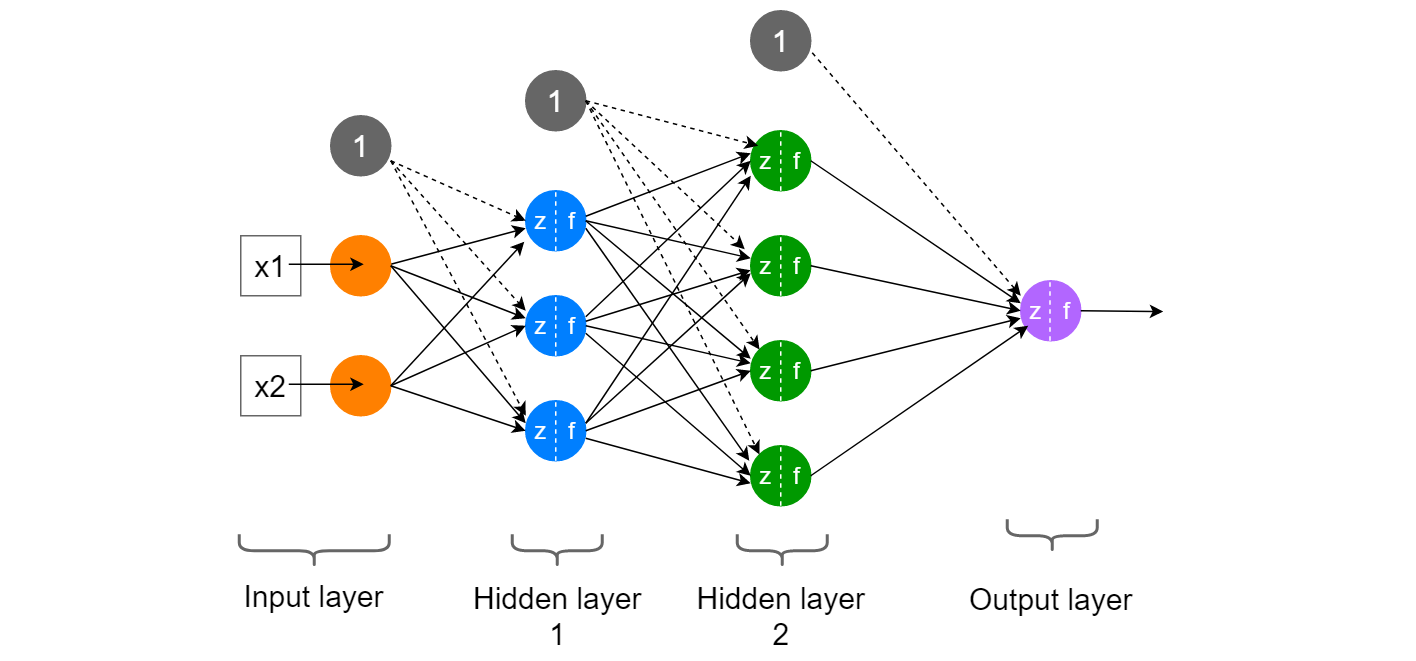
\includegraphics[width=\textwidth]{images/figure1.png}
    \caption{A typical Artificial Neural Network}
    \label{fig:1}
\end{figure}

\section{Background}
Artificial Neural Networks (ANNs) are computational models inspired by the structure and function of biological neural networks in the human brain. The idea of mimicking biological neurons dates back to the 1940s with the introduction of the \textbf{McCulloch-Pitts neuron model}, which laid the foundation for modern neural networks.\cite{mcculloch1943logical} Early research explored how networks of artificial neurons could compute logic functions and recognize patterns.\\

By the 1980s, the \textbf{backpropagation algorithm}, introduced by Rumelhart, Hinton, and Williams, marked a turning point by enabling efficient training of multi-layer networks.\cite{rumelhart1986learning} This innovation fueled interest in neural networks for tasks such as image recognition, speech processing, and robotics.\\

Despite their promise, neural networks struggled during the 1990s due to computational limitations and the dominance of simpler models like support vector machines (SVMs). However, the resurgence of interest in the 2010s, termed the \textbf{"deep learning revolution"}, was driven by three factors:
\begin{itemize}
    \item Availability of large datasets (e.g., ImageNet)
    \item Advancements in computational power (e.g., GPUs and TPUs).
    \item Development of new architectures and techniques, such as convolutional neural networks (CNNs) and recurrent neural networks (RNNs).\cite{lecun2015deep}\cite{krizhevsky2012imagenet}
\end{itemize}

\section{Applications of Neural Networks}
Neural networks are used across diverse domains, revolutionizing traditional methods with their ability to learn from data and generalize well. Prominent applications include:
\begin{itemize}
    \item \textbf{Image Recognition}: Tasks like facial recognition and object detection rely on CNNs to extract hierarchical features from images.\cite{lecun2015deep}
    \item \textbf{Natural Language Processing (NLP)}: Models like transformers power language models such as ChatGPT and BERT, enabling applications like sentiment analysis, translation, and summarization.\cite{vaswani2017attention}
    \item \textbf{Healthcare}: ANN-based solutions are applied for early diagnosis of diseases, drug discovery, and personalized treatment recommendations.\cite{esteva2017dermatologist}
    \item \textbf{Autonomous Systems}: Self-driving cars use neural networks to process sensor data for navigation and decision-making.\cite{bojarski2016end}
\end{itemize}

and many more...

\section{Importance of Neural Networks in Modern AI}
Neural networks form the backbone of modern AI, offering unparalleled flexibility and scalability for solving complex problems. Their key advantages include:
\begin{enumerate}
    \item \textbf{Automatic Feature Extraction}: Unlike traditional machine learning algorithms, ANNs can automatically learn hierarchical features from raw data.
    \item \textbf{Non-linearity}: Through activation functions, ANNs can model complex, non-linear relationships in data.
    \item \textbf{Scalability}: Modern architectures, such as deep neural networks, allow scaling to billions of parameters for solving real-world problems at scale.
\end{enumerate}

However, ANNs also have limitations, such as their need for large amounts of labeled data, computational intensity, and susceptibility to overfitting. Addressing these challenges remains a significant focus in the AI research community.\cite{goodfellow2016deep}

             % Introduction
\chapter{Logistic Regression}\label{chp:2}

\section{Fundamentals of Logistic Regression}
Logistic regression is a statistical method for binary classification, where the goal is to predict a binary outcome (e.g., success/failure, $0/1$) based on one or more input variables. Unlike linear regression, logistic regression outputs probabilities by applying a \textbf{sigmoid function} to a linear combination of the inputs.\\

Consider a set $\mathcal{S} = \{(x^{(1)}, y^{(1)}), \dots, (x^{(m)}, y^{(m)})\} \subseteq \mathcal{X} \times \mathcal{Y}$ of \textcolor{blue}{\emph{training data}} with $\mathcal{X} \subseteq \mathbb{R}^d$ and $\mathcal{Y}=\{0,1\}$. In this set, every $x^{(i)}$ represents an \textcolor{blue}{\emph{object}} and the corresponding \textcolor{blue}{\emph{label}} $y^{(i)}$ indicates which one of two possible cases the object belongs to. \textcolor{blue}{\emph{Binary Classification}} describes the search for a map $h_{\theta}: \mathcal{X} \rightarrow \mathcal{Y}$ parametrized by $\theta \in \Theta$, which maps every object $x \in \mathcal{X}$ to a label $y \in \mathcal{Y}$.\\

In this context, we call $\Theta$ the \textcolor{blue}{\emph{parameter space}} and $h_{\theta}$ a \textcolor{blue}{\emph{hypothesis}}. A particular approach for identifying suitable hypotheses for binary classification problems is \textcolor{blue}{\emph{logistic regression}} (for example, see \cite[chapter 4.3.2]{bishop2006pattern} and \cite[chapter 5.7.1]{goodfellow2016deep}), which we discuss in what follows.

\begin{definition}[Sigmoid function]
The function
\begin{equation}
    \sigma : \mathbb{R} \to (0, 1), \quad \sigma(z) := \frac{1}{1 + e^{-z}}
    \label{eqn:1}
\end{equation}
is called a \textcolor{blue}{\emph{sigmoid function}} or (more general) \textcolor{blue}{\emph{logistic function}}.
\end{definition}

Here, $z = w^\top x + b$, where $w$ represents the weights, $x$ the input features, and $b$ the bias term.\\

\textbf{Key features}:
\begin{itemize}
    \item \textbf{Output Interpretation}: The sigmoid function ensures outputs lie in the range $(0, 1)$, making them interpretable as probabilities.
    \item \textbf{Decision Boundary}: The model predicts class $1$ if $\sigma(z) \geq 0.5$ and class $0$ otherwise. This results in a decision boundary defined by the hyperplane $w^\top x + b = 0$.\cite{hastie2009elements}
\end{itemize}

\section{Learning as an Optimization Problem}
From a statistical perspective, logistic regression models the probability distribution of the data as a \textbf{Bernoulli distribution} with parameter $\sigma(z)$. The model is trained by maximizing the \textbf{likelihood function}, which represents the probability of observing the given training data under the model parameters.\\

\textbf{Maximum Likelihood Viewpoint}\\

The goal is to come up with a distribution on $\mathcal{X} \times \mathcal{Y} \subseteq \mathbb{R}^d \times \{0,1\}$ that “prioritizes” the training data. In other words, it should assign small (or even zero) values to an elementary event $(x, y) \in \mathcal{X} \times \mathcal{Y}$, where $y$ is \textbf{not} the correct label of $x$. In
order to approach this task, we consider the family

\begin{equation}
    \mathcal{D}_{Mod}(y|x;\theta) := \sigma(w^\top x +b)^y \cdot (1 - \sigma(w^\top x +b))^{1-y}, \quad \theta = (w, b) \in \Theta
    \label{eqn:2}
\end{equation}

of \textcolor{blue}{\emph{model}} measures on $\mathcal{X} \times \mathcal{Y} \subseteq \mathbb{R}^d \times \{0,1\}$ parametrized by $\Theta= \mathbb{R}^d \times \mathbb{R}$. We have

\begin{equation}
    \mathcal{D}_{\text{Mod}}(y \mid x; \theta) =
    \begin{cases} 
        \sigma(w^\top x + b), & \text{if } y = 1 \\
        1 - \sigma(w^\top x + b), & \text{if } y = 0
    \end{cases}
    \label{eqn:3}
\end{equation}

and $\mathcal{D}_{\text{Mod}}(\cdot|x;\theta)$ is a Bernoulli probability distribution with parameter $\sigma(w^\top x + b)$. This parameter hence represents (in our model) the probability that $y=1$ is the correct label for a given $x$, while the probability that $y=0$ is the correct label for $x$ equals $1 - \sigma(w^\top x + b)$.\\

The problem of \emph{Maximum Likelihood Estimation} seeks a parameter $\theta=(w,b)$ such that the probability of observing $\mathcal{S}$ is maximal (among $\mathcal{D}_{\text{Mod}}(\cdot|\cdot;\theta)$). Thus, given \emph{pairwise independent} random variables $X^1, \dots, X^m$ on $\mathcal{X} \times \mathcal{Y}$ distributed according to $\mathcal{D}_{\text{Mod}}(\cdot|\cdot;\theta)$, we have to maximize the \textcolor{blue}{\emph{likelihood function}}:

\begin{equation}
    \begin{aligned}
    \mathcal{L}(\theta) &:= \mathbb{P}(\{X^1 = (x^{(1)}, y^{(1)}), \dots, X^m = (x^{(m)}, y^{(m)})\}), \quad \theta=(w,b)\\
    & \overset{\text{i.i.d.}}{=} \prod_{i=1}^{m}\mathcal{D}_{\text{Mod}}(y^{(i)}|x^{(i)};\theta)\\
    & = \prod_{i=1}^{m}\sigma(w^\top x^{(i)} + b)^{y^{(i)}} \cdot (1 - \sigma(w^\top x^{(i)} + b))^{1 - y^{(i)}}
    \end{aligned}
    \label{eqn:4}
\end{equation}

Equivalently, we can minimize the negative log of the likelihood function as below, which gives us the \textcolor{blue}{\emph{cross entropy loss function}}:
\begin{equation}
    \begin{aligned}
    -\ln \mathcal{L}(\theta) &= -\ln(\prod_{i=1}^{m}\mathcal{D}_{\text{Mod}}(y^{(i)}|x^{(i)};\theta))\\
    &= -\sum_{i=1}^{m}\ln(\mathcal{D}_{\text{Mod}}(y^{(i)}|x^{(i)};\theta))\\
    &= -\sum_{i=1}^{m}\ln(\sigma(w^\top x^{(i)} + b)^{y^{(i)}} \cdot (1 - \sigma(w^\top x^{(i)} + b))^{1 - y^{(i)}})\\
    &= -\sum_{i=1}^{m}[\ln(\sigma(w^\top x^{(i)} + b)^{y^{(i)}})+ \ln(1 - \sigma(w^\top x^{(i)} + b))^{1 - y^{(i)}})]\\
    &= -\sum_{i=1}^{m}[y^{(i)}\ln(\sigma(w^\top x^{(i)} + b))+(1-y^{(i)})\ln(1 - \sigma(w^\top x^{(i)} + b))]
    \end{aligned}
    \label{eqn:5}
\end{equation}


The parameters $w$ and $b$ are learned by minimizing this loss using optimization algorithms such as gradient descent.\cite{murphy2012machine}\\

Thus, a maximum likelihood estimator $\hat{\theta} \in \Theta$ is a solution to the following non-linear optimization problem:
\begin{equation}
    -\ln \mathcal{L}(\hat{\theta}) = \min_{\theta \in \Theta} - \ln \mathcal{L}(\theta)
    \label{eqn:6}
\end{equation}

\section{From the Model Distribution to the Hypothesis} \label{hypothesis}

Once the parameter $\theta=(w,b)$ is fixed, we apply the hypothesis
\begin{equation}
    h_{\theta}(x) :=
    \begin{cases} 
        1, & \text{if } \mathcal{D}_{\text{Mod}}(1|x;\theta) \geq 0.5 \\
        0, & \text{else}
    \end{cases}
    \label{eqn:7}
\end{equation}

to an object $x \in \mathcal{X}$ with (potentially) unknown label $y \in \mathcal{Y}$. That means we apply, based on our model distribution, “the most likely” label to $x$ (which one can consider to be the natural or intuitive thing to do). In case that $x$ is on the boundary region $\mathcal{D}_{\text{Mod}}(1|x;\theta) = \mathcal{D}_{\text{Mod}}(0|x;\theta) = 0.5$, where both labels have the same probability, we need to take a decision of favoring one label.\\

Due to the fact that $\sigma(0)=0.5$ and that $\sigma$ is a strictly monotonically increasing function (refer Figure \ref{fig:4}), we conclude that the sets $\{ x \in \mathcal{X} \mid h_{\theta}(x) = 1 \}$ and $\{ x \in \mathcal{X} \mid h_{\theta}(x) = 0 \}$ are separated by the hyperplane $\mathcal{E} := \{ x \in \mathcal{X} \mid w^\top x + b = 0 \}$. Therefore, our decision rule \ref{eqn:7} is described as:

\begin{equation}
    h_{\theta}(x) :=
    \begin{cases} 
        1, & \text{if } w^\top x + b \geq 0 \\
        0, & \text{else } w^\top x + b < 0
    \end{cases}
    \label{eqn:8}
\end{equation}

and we call the hyperplane $\mathcal{E}$ the \textcolor{blue}{\emph{decision boundary}} (see Figure \ref{fig:2}).

\begin{figure}[h!]
    \centering
    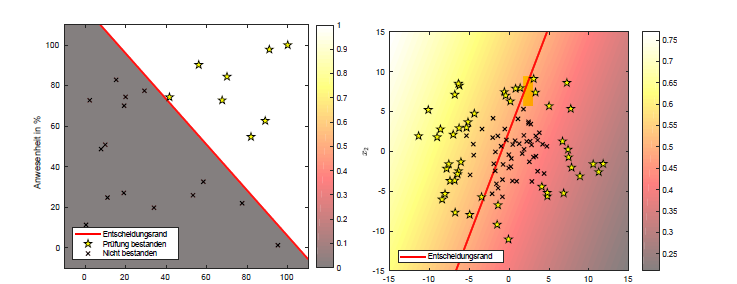
\includegraphics[width=1.1\textwidth]{images/figure2.png}
    \caption{
        \textbf{Left:} Example for a logistic regression on linearly separable data.
        \textbf{Right:} Example for logistic regression on linearly non-separable data. The computed hypothesis achieves only an accuracy of 68\% on the training data. The coloring represents the values of $\sigma(w^\top x + b)$.
    }
    \label{fig:2}
\end{figure}

Figure \ref{fig:3} shows how logistic regression typically works to predict the label.

\begin{figure}[h!]
    \centering
    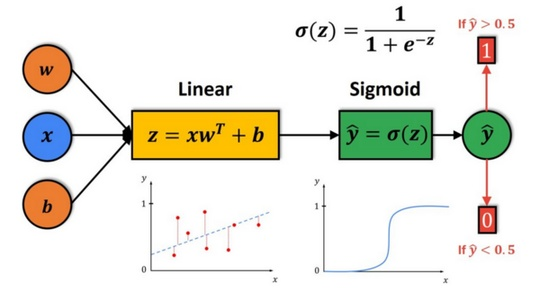
\includegraphics[width=0.75\textwidth]{images/figure3.jpg}
    \caption{How Logistic Regression typically works}
    \label{fig:3}
\end{figure}

\section{Machine Learning Formulation}
Now we embed the adopted statistical point of view into the context of machine learning. We take a closer look at the summand in our target function \ref{eqn:5}, which we have to minimize (refer \ref{eqn:6}).

\begin{definition}[Cross entropy loss function]
The function
\begin{equation}
    \ell : \{0,1\} \times \{0,1\} \rightarrow \mathbb{R}, \quad \ell(y, \hat{y}):= -y\ln (\hat{y}) - (1-y)\ln(1 - \hat{y})
    \label{eqn:9}
\end{equation}
is called \textcolor{blue}{\emph{cross entropy loss function}}.
\end{definition}

Note that $\ell(y, \hat{y})$ is nothing but the cross entropy between Bernoulli
distributions with parameters $y$ and $\hat{y}$. Using this cross-entropy loss function, we reformulate the minimization problem \ref{eqn:6} as:
\begin{equation}
    \min_{\theta = (w,b) \in \Theta} \frac{1}{m} \sum_{i=1}^{m} \ell (y^{(i)}, \sigma(w^\top x^{(i)}+b))
    \label{eqn:10}
\end{equation}

\begin{figure}[h!]
    \centering
    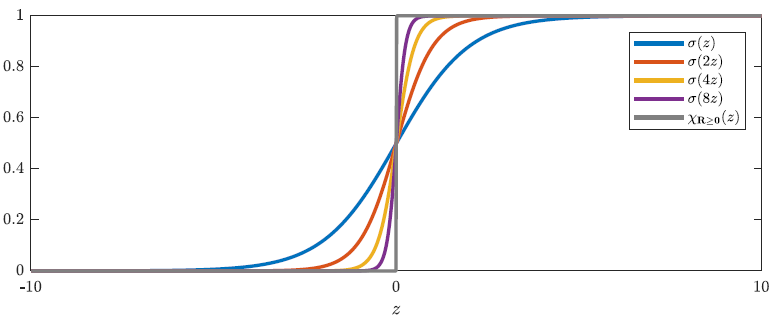
\includegraphics[width=\textwidth]{images/figure4.png}
    \caption{The sequence $(\sigma(nz))_{n \in \mathbb{N}}$ converges uniformly to a characteristic function on $\mathbb{R} \setminus \{0\}$.}
    \label{fig:4}
\end{figure}

\fbox{%
    \parbox{\textwidth}{%
        \textbf{NOTE}: The additional factor $\frac{1}{m}$ does not change the optimal points (i.e., maximum Likelihood estimators $\hat{\theta}$). We can interpret every summand in (\ref{eqn:10}) as the distance between a known target value (i.e., label) $y^{(i)}$ and a prediction $\sigma(w^ \top x^{(i)} + b)$ based on our model. The more accurate our model makes predictions on the training data, the smaller are the individual values $\ell (y^{(i)}, \sigma(w^\top x^{(i)}+b))$ contributing to the target function of the optimization problem.
    }%
}

\section{Minimizing Risks}
Minimizing sums of the form (\ref{eqn:10}) is a (type of) problem that one encounters regularly in the context of machine learning. To make our goal, the prediction of class membership of objects $x \in \mathcal{X}$ with unknown labels, more precise, we investigate another alternative formulation of (\ref{eqn:10}).\\

\begin{definition}[Empirical Risk Distribution]
The distribution $\hat{\mathcal{D}}$ with
\begin{equation}
    \hat{\mathcal{D}}(A) := \frac{1}{m}\sum_{i=1}^{m}\delta_{(x^{(i)}, y^{(i)})}(A)
    \label{eqn:11}
\end{equation}
on $\mathcal{X} \times \mathcal{Y}$ and
\begin{equation}
    \delta_{(x^{(i)}, y^{(i)})}(A) =
    \begin{cases} 
        1, & \text{if } (x^{(i)}, y^{(i)}) \in A \\
        0, & \text{otherwise}
    \end{cases}
    \label{eqn:12}
\end{equation}
is called \textcolor{blue}{\emph{empirical distribution}} with respect to $\mathcal{S}$.
\end{definition}

We can formulate the target function in (\ref{eqn:10}) as an expected value as below:
\begin{equation}
    \frac{1}{m} \sum_{i=1}^{m} \ell (y^{(i)}, \sigma(w^\top x^{(i)}+b)) = \mathbb{E}_{(x,y) \sim \hat{\mathcal{D}}}\ell (y, \sigma(w^\top x+b)) =: \mathcal{J}(\theta)
    \label{eqn:13}
\end{equation}

Thus, \ref{eqn:13} is also called the \textcolor{blue}{\emph{empirical risk}} and the computation of $\hat{\theta}$ via the problem
\begin{equation}
    \mathcal{J}(\hat{\theta}) = \min_{\theta \in \Theta} \mathcal{J}(\theta)
    \label{eqn:14}
\end{equation}

which is equivalent to (\ref{eqn:10}), is called \textcolor{blue}{\emph{empirical risk minimization}}.\\

However, our goal is not minimizing the empirical risk, but rather minimizing the \textcolor{blue}{\emph{true risk}}
\begin{equation}
    \mathbb{E}_{(x,y) \sim \mathcal{D}}\ell (y, \sigma(w^\top x+b)) =: \mathcal{J}^*(\theta),
    \label{eqn:15}
\end{equation}

i.e., we have to find
\begin{equation}
    \theta^* \in \argmin_{\theta \in \Theta} \mathcal{J}^*(\theta)
    \label{eqn:16}
\end{equation}

But, we do not know the underlying distribution $\mathcal{D}$, and hence we cannot solve
the problem (\ref{eqn:16}) directly. Empirical risk minimization can therefore be interpreted as \emph{replacing} the unknown (true) distribution $\mathcal{D}$ in (\ref{eqn:16}) by the empirical distribution $\hat{\mathcal{D}}$, which is induced by our sample $\mathcal{S}$.


\section{Limitations of Logistic Regression: Linear Separability} \label{limitations}
While logistic regression is simple and interpretable, it has significant limitations that restrict its applicability.

\subsection{Linear Decision Boundaries}
Logistic regression assumes that the classes can be separated by a linear boundary. For datasets with complex, non-linear relationships, this assumption leads to poor performance.\\

In section \ref{hypothesis}, we interpreted logistic regression as learning a hyperplane $\mathcal{E}$ that separates the space $\mathcal{X} = \mathbb{R}^d$ in two half-spaces $\{x \in \mathcal{X}\text{ }|\text{ }h_{\theta}(x) =0 \}$ and $\{x \in \mathcal{X}\text{ }|\text{ }h_{\theta}(x) =1 \}$. If the hyperplane, which we learn, classifies all objects in our training data correctly (i.e., the training data is linearly separable), then we have $h_{\theta}(x^{(i)})=y^{(i)}$ for all training examples. If we define $\mathcal{X}_{\mathcal{S}} := \{x \in \mathcal{X}\text{ }|\text{ }\exists y \in \mathcal{Y} : (x,y) \in \mathcal{S} \}$, then it follows immediately that the sets
\begin{equation}
    \begin{aligned}
        \mathcal{X}_0 &:= \{x^{(i)} \in \mathcal{X}_{\mathcal{S}}\text{ }|\text{ }y^{(i)}=0 \} \subset \{x \in \mathcal{X}\text{ }|\text{ }h_{\theta}(x)=0 \}\\
        \mathcal{X}_1 &:= \{x^{(i)} \in \mathcal{X}_{\mathcal{S}}\text{ }|\text{ }y^{(i)}=1 \} \subset \{x \in \mathcal{X}\text{ }|\text{ }h_{\theta}(x)=1 \}
    \end{aligned}
    \label{eqn:17}
\end{equation}
are also linearly separable. Note that the property to be linearly separable depends only on the sample $\mathcal{S}$ and is hence \emph{independent} of the hyperplane which we learned. This means in particular that, if two sets $\mathcal{X}_0$ and $\mathcal{X}_1$ cannot be separated linearly, then it is \emph{impossible} to learn a hyperplane via
logistic regression that classifies all training data correctly. In other words, we obtain $h_{\theta}(x^{(i)}) \neq y^{(i)}$ for a positive percentage of our training data (see right-hand side of Figure \ref{fig:5}).

\begin{figure}[h!]
    \centering
    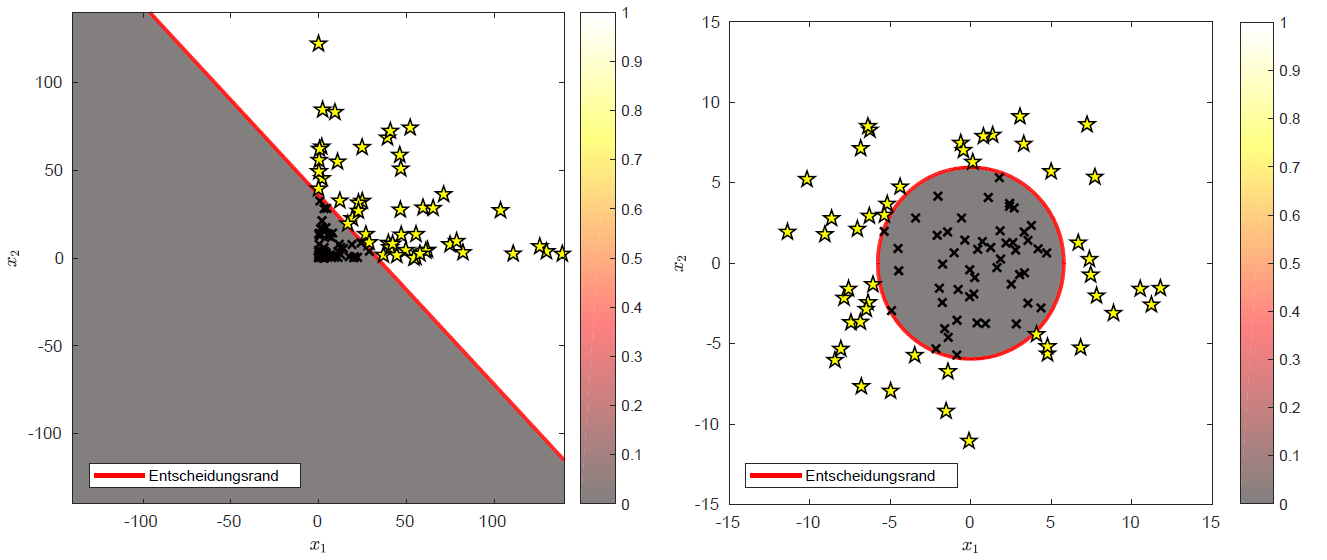
\includegraphics[width=\textwidth]{images/figure5.png}
    \caption{
        Example of logistic regression with basis functions applied to data, which is not linearly separable $\phi_1(x) = x_1^2$ and $\phi_2(x) = x_2^2$. The computed hypothesis is $100\%$ accurate on the training data. The coloring represents the values of $\sigma(w^\top \phi(x)+b)$. On the left-hand side one can see the feature vectors $\phi^{(i)}$, which are linearly separated by the decision boundary $\{\phi \in \mathbb{R}^n\text{ }|\text{ }w^ \top\phi+b =0\}$. On the right-hand side one can see the original objects $x^{(i)}$, which are separated by the nonlinear decision boundary $\{x \in \mathbb{R}^d\text{ }|\text{ }w^ \top\phi(x)+b =0\}$ given by the basis functions.
    }
    \label{fig:5}
\end{figure}

\subsection{Feature Engineering Dependency}
In order to learn nonlinear decision boundaries in the context of logistic regression, one can use \textcolor{blue}{\emph{basis functions}} (see \cite[chapter 4.3.2]{bishop2006pattern}), $\phi_1, \dots, \phi_n : \mathbb{R}^d \rightarrow \mathbb{R}$. Every one of these basis functions $\phi_j(x)$ can be nonlinear in $x$. We can interpret these functions as representing a particular \emph{pattern} of the object $x$. Thus, we call the vectors
\begin{equation}
    \phi^{(i)} := \phi(x^{(i)}) := 
    \begin{pmatrix}
        \phi_1(x^{(i)}) \\
        \vdots \\
        \phi_n(x^{(i)})
    \end{pmatrix}
    \label{eq:18}
\end{equation}

also \textcolor{blue}{\emph{feature vectors}}. The feature vector $\phi^{(i)}$ represents the object $x^{(i)}$ via the extracted pattern $\phi_1(x^{(i)}), \dots, \phi_n(x^{(i)})$, which are nothing but the coordinates of $\phi^{(i)}$. If the basis functions are given (or chosen), then we can apply logistic regression as described before with the crucial
difference that we now use training data $\{(\phi^{(1)}, y^{(1)}), \dots, (\phi^{(m)}, y^{(m)}) \} \subseteq \mathbb{R}^n \times \{0, 1\}$.\\

Note that the cardinality $n$ of the basis functions does not need to coincide with the dimension $d$ of the objects $x$.\\

If we apply logistic regression to data, which was transformed via basis functions, then we need to adjust the number of parameters. Now, we have $\theta = (w, b) \in \mathbb{R}^n \times \mathbb{R}$. Thus, possible hypotheses are of the form

\begin{equation}
    h_{\theta}(x) =
    \begin{cases} 
        1, & \text{if } w^ \top \phi(x) + b \geq 0 \\
        0, & \text{if } w^ \top \phi(x) + b < 0
    \end{cases}
    \label{eqn:19}
\end{equation}

with associated decision boundaries $\{x \in \mathcal{X} \text{ }|\text{ }w^\top \phi(x) +b =0 \}$.

\subsection{High-dimensional Data}
In cases where the number of features is very large (e.g., image data), logistic regression struggles due to overfitting or computational inefficiency.

\subsection{Multi-class Classification}
Logistic regression inherently handles only binary classification. Extending it to multi-class problems (e.g., through one-vs-rest or softmax regression) increases complexity.


\section{Role of Basis Functions in Logistic Regression}
As we have seen in section \ref{limitations}, to address the limitation of linear decision boundaries, \emph{basis functions} are introduced. These are transformations of the input features that allow logistic regression to model non-linear relationships(see \cite[chapter 4.3.2]{bishop2006pattern})\\

\vspace{10mm}
\textbf{TO BE CONTINUED... }
\vspace{10mm}





\textbf{Example: Polynomial Basis Functions}
Consider a dataset where two classes are not linearly separable in the original feature space. By transforming the features using quadratic functions (e.g., $x_1^2$, $x_2^2$, $x_1x_2$), we can project the data into a higher-dimensional space where it becomes linearly separable.\\

However, this approach has challenges:
\begin{itemize}
    \item \textbf{Choosing the Right Basis Functions}: It requires domain knowledge or trial-and-error to select suitable transformations.
    \item \textbf{Dimensional Explosion}: The number of basis functions grows exponentially with the degree of the polynomial and the number of input features. For example, a second-degree polynomial in 400 features produces over 80,000 basis functions.\cite{hastie2009elements}
\end{itemize}

\section{Transition to Neural Networks}
Artificial Neural Networks (ANNs) solve the limitations of logistic regression by \textbf{learning the basis functions automatically}. Instead of manually defining transformations, ANNs use layers of neurons to hierarchically extract features from the data.\\

\textbf{How ANNs Improve on Logistic Regression}:
\begin{enumerate}
    \item \textbf{Automatic Feature Learning}:
    \begin{itemize}
        \item Neural networks learn non-linear transformations directly from the data.
        \item For example, convolutional layers in CNNs extract spatial patterns like edges and shapes.
    \end{itemize}
    \item \textbf{Scalability}:
    \begin{itemize}
        \item ANNs can scale to millions of parameters, enabling them to model high-dimensional data efficiently.
    \end{itemize}
    \item \textbf{Universal Approximation}:
    \begin{itemize}
        \item A neural network with sufficient depth and width can approximate any function, linear or non-linear.
    \end{itemize}
    \item \textbf{Multi-Class Capability}:
    \begin{itemize}
        \item Using the \textbf{softmax activation function}, ANNs natively support multi-class classification tasks.
    \end{itemize}
\end{enumerate}
Thus, ANNs represent a significant advancement over traditional logistic regression, paving the way for breakthroughs in deep learning.











% Bibliography Section
% --------------------
% \bibliographystyle{ieeetr}            % Style for bibliography
% \bibliographystyle{unsrt}             % Style for bibliography
\bibliographystyle{alpha}               % Style for bibliography
\bibliography{bibliography}             % References in bibliography.bib


\end{document}
